\documentclass[12pt,a4paper,leqno]{report}
\usepackage[utf8]{inputenc}
\usepackage[norsk]{babel}
\usepackage{amsmath}
\usepackage{amsfonts}
\usepackage{amssymb}
\usepackage{graphicx}
\usepackage{float}
\usepackage{tikz}

\usepackage[left=2cm,right=2cm,top=2cm,bottom=2cm]{geometry}
\author{Krister Borge, Fransis Uno Nyka Kolstø}
\title{Labrapport \\ \small{prelab}}

\begin{document}
\maketitle
\textbf{Oppgave 1.1}


Vi koblet opp spenningskilden og kondensatoren og voltmeteret over kondensetaren. Vi så at spenningen over kondensatoren gikk til $V_0$ umiddelbart. 
Så koblet vi av spenninga og målte spenningen med $\Delta t=5s$\\
Vi så at kondensatoren falt til halv spenning på under et minutt, derofr økte vi antall målepunkter og målte i kun 2 minutter.
\begin{figure}[H]
\caption{Oppgave 1.1 Logaritmisk plot av spenning over tid}
\centering
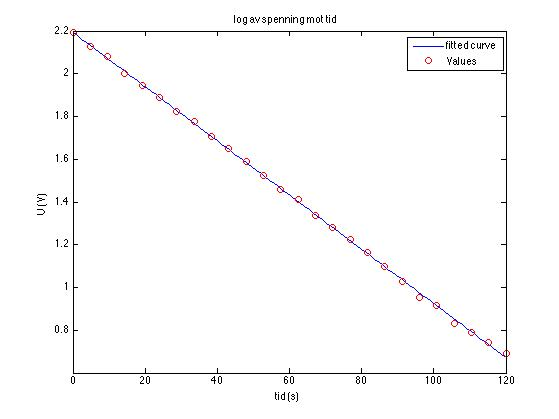
\includegraphics[width=\textwidth]{gjennomforing/oppgave11/oppgave11LOGUvT.jpg}
\end{figure}

\begin{figure}[H]
\caption{Oppgave 1.1 Logaritmisk plot av spenning over tid}
\centering
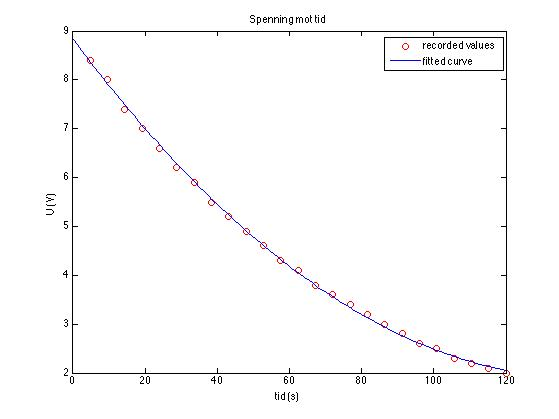
\includegraphics[width=\textwidth]{gjennomforing/oppgave11/oppgave11UvT.jpg}
\end{figure}

For å finne R fant vi tidskontstanten $\tau$ (første element i førstegradspolynomet fra matlabs ployval) for kretsen og delte på kondensatorens verdi.Denne var på 8.3$\mu$ F.

\begin{verbatim}
function []=lab1oppgave11(min, max, datapunkt,degree)
x = linspace(min,max,length(datapunkt));
y=datapunkt;

p = polyfit(x, datapunkt,degree);

x1 = linspace(min,max);
y1 = polyval(p,x1);
%plot
figure
plot(x,y,'or',x1,y1,'b')
title('Spenning mot tid')
xlabel('tid (s)')
ylabel('U (V)')
legend('recorded values', 'fitted curve')


lny=log(datapunkt);
p2=polyfit(x,lny,1)
y2=polyval(p2,x1);
figure()
plot(x1,y2,'b',x,lny, 'or')
xlabel('tid (s)')
ylabel('U (V)')
legend('fitted curve','Values ')
title('log av spenning mot tid')
%finner \tau og R_internal
tau=abs(p2(1))
F=8.3e-6
R=tau/F
end
\end{verbatim}

\begin{verbatim}
tau =  0.0122
F = 8.3000e-06
R = 1.4714e+03
\end{verbatim}



\textbf{Prelab-Oppgave 1}

Spenningen over en oppladet kondensator med C=1 $\mu$ F
som er koblet til inngangen på et voltmeter halveres på 20 sekunder. Hva er indre resistansen til voltmeteret?\\
Kondensatoren og voltmeteret skaper denne kretsen:
\begin{figure}[H]
\caption{RC-krets}
\centering
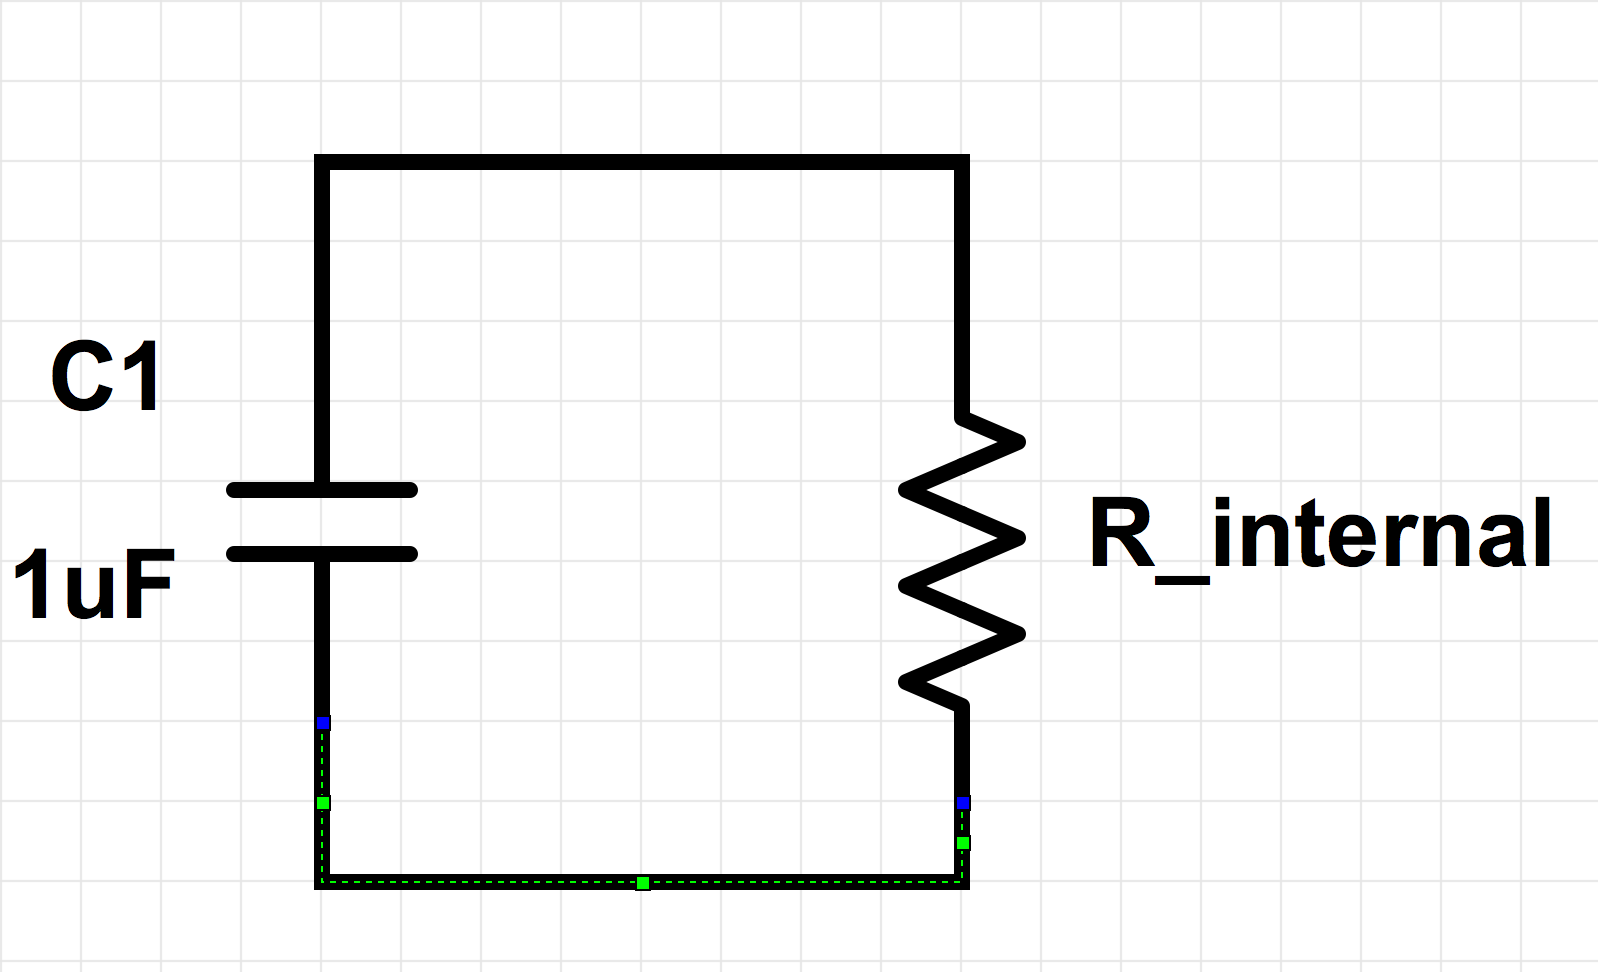
\includegraphics[width=\textwidth]{RC-cirquit.jpg}
\end{figure}
Jeg veit at $\tau=$RC. jeg veit også halveringstiden til kondensatoren som er 20 sekunder. Etter  1 $\tau$  er kondensatoren på 37\% av maks spenning. etter $t=20$ sekunder er spenningen lik $\frac{V_{max}}{2}$.
\begin{equation}
V(t)=V_0e^{-t/R_{internal}C}
\end{equation}

For RC-kretser gjelder:
\begin{equation}
\tau=RC
\end{equation}
men jeg har kondensator verdien og løser for R:
\begin{equation}
\ln(2)=\frac{t}{RC}
\end{equation}
\begin{equation}
\ln(2)=\frac{20}{RC}
\end{equation}
\begin{equation}
\ln(2)=\frac{20}{R1 \mu F}
\end{equation}
\begin{equation}
\ln(2)R=\frac{\frac{0,2}{10^{-6} F}}{\ln{2}}=\frac{2000000}{\ln(2)}=28853900,816=2,8853900816\mathsf{M}\Omega
\end{equation}

Der $V_0$ er den initielle spenningen i kondensatoren.
Jeg har også at $Q_{max}=CV_{max}$
$F=\frac{Q}{V}$ 
\pagebreak

\textbf{Oppgave 1.2}

Når spenningskilden er koblet til blir det en konstant ladning på kondensatoren. Når denne spenningen fjernes er det kun ladningene i kondensatoren som skaper spenning i kretsen. For hvert tidsteg går strømmen fra den ene siden til den andre av kondenstatoren og dette fører til at spenningen minker.  

\textbf{Oppgave 2.1}

Dekaderesistoren ble koblet til en spenningskilde, deretter koblet vi et voltmeter og ampermeter(i 100 mA inngangen) over dekaderessistoren for å måle strømmen og spenningen ved forskjellige motstander. Avmålingene ble satt in I hvert sitt array I MATLAB, og det ble brukt polyval og polyfit for å lage tilpassede grafer.

Polyval I første grad ga oss et stigningstall på 11.5, som tilsvarer den interne resistansen. (11.5$\Omega$)

\begin{figure}[H]
\caption{oppgave 2.1 : Motstander}
\centering
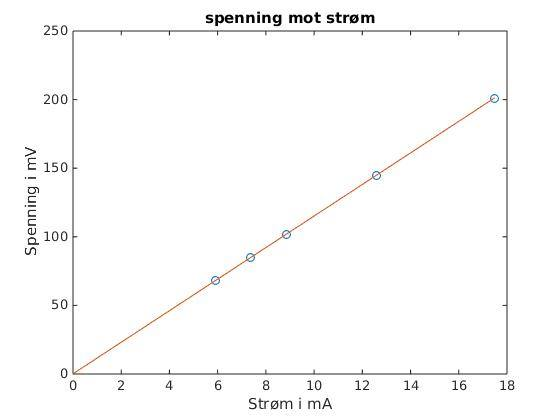
\includegraphics[width=\textwidth]{gjennomforing/oppgave21/fransislab1oppgave21.jpg}
\end{figure}


\textbf{Oppgave 2:} 

Lag et MATLAB-skript basert på metodene polyfit og polyval som tilpasser en linje til et sett med datapunkter x,y og viser punktene og den tilpassede linjen på en figur. Dette skriptet kan også brukes i labøvelse 3(Hall-effekt).

\begin{figure}
\caption{Matlabskript}
\begin{verbatim}
function []=lab1oppgave2(min, max, datapunkt,degree)
x = linspace(min,max,length(datapunkt));
y=datapunkt;
%
p = polyfit(x, datapunkt,degree);

x1 = linspace(min,max);
y1 = polyval(p,x1);
%plot
figure
plot(x,y,'or',x1,y1,'b')
title('Values and fitted curve')
legend('recorded values', 'fitted curve')

end
\end{verbatim}
\end{figure}
Dette kallet: 
\begin{verbatim}
>> lab1oppgave2(0,9,[1,2,5,7,16,19,11,15,11,19,11,15,14,19,11,15,13],7)
\end{verbatim}
gir dette plottet:
\begin{figure}[H]
\caption{Test av matlabskript}
\centering
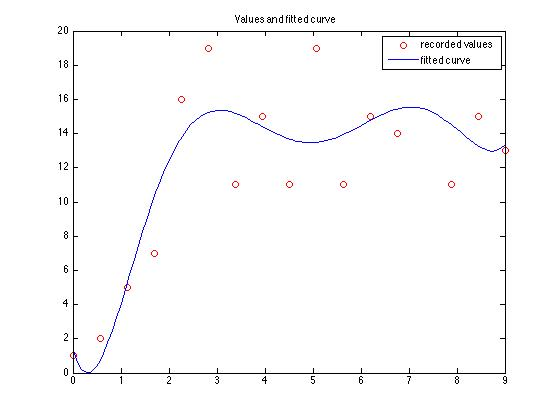
\includegraphics[width=\textwidth]{curvefittertest.jpg}
\end{figure}

\textbf{Oppgave 3.1:}
Vi undersøkte peltier-elementet nøye. Først koblet vi det til voltmeter. Vi observerte at ved å varme opp flatene på peltier-elementet skapte den en spenning. Vi koblet den så på spenningskilden, da ble den kald på den ene siden og litt lunka på den andre. 

\textbf{Oppgave 3.1:}

Vi fylte opp kobberkoppen med varmt vann. Plasserte elementet mellom kobberklumpen og koppen. Deretter paralellkoblet vi peltierelementet (generatoren) med voltmeteret og dekaderesitoren. så tok vi mplinger for verdiene satt i oppgaveteksten:
\begin{figure}[H]
\caption{}
\centering
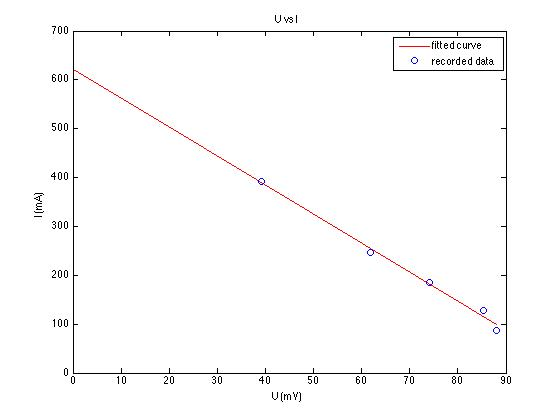
\includegraphics[width= \textwidth]{gjennomforing/oppgave31/lab1oppgave31.jpg}
\end{figure}
\textbf{Oppgave 2.4:} 

Firepunktsmåling av resistansen.
Her skal vi måle en strøm og spenning over en resistanse. 

Motstanden i måleinstrumentene har noe å si når man måler strøm. Den store resistansen i ameteret og den lille i voltmeteret.



\begin{figure}[H]
	\caption{}
	\centering
	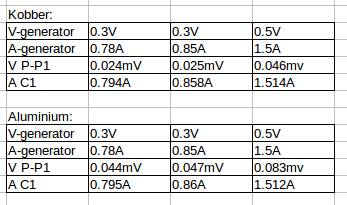
\includegraphics[scale=1]{gjennomforing/oppgave4.jpg}
	\end{figure}
 
\textbf{prelab Oppgave 3:} 

Finn et uttrykk for $\mathbf{B}$ dersom vi dreier spolen med konstant vinkelhastighet $\omega$ og måler den maksimale verdien $\epsilon_0$ for $\epsilon(t)$. Hva er forholdet mellom 
$\omega$ og $t_0-t_1$?

Der spolens $N$ er spolens vindingstall og $A$ er spolens areal.
orientasjonen er slik at $\Phi(t_1)=NAB$ og 
\begin{equation}
2NAB=\int_{t1}^{t2}\epsilon(t)dt
\end{equation}
Jeg kan så se på hver del for seg:
\begin{equation}
\Phi=2NAB\omega(t_1)=2NAB\sin(omega*t)
\end{equation}
Et utrykk for \textbf{B} kan da være:
\begin{equation}
\mathbf{B}=\frac{\Phi(t_1)}{2NA\sin(omega*t)}
\end{equation}
Der $\Phi(T)$ kan utrykkes ved
\begin{equation}
-\int_{t1}^{t2}\epsilon(t)dt
\end{equation}

Amperes lov sier:
\begin{equation}
\oint \mathbf{B} ds=\mu_0I
\end{equation}
$\mu_0$ er permitiviteten.

Forholdet $\omega/t_1-t_2$:
\begin{equation}
\omega=\frac{2 \pi} {T}
\end{equation}

\begin{equation}
B=\frac{\epsilon_max \Delta t} {\pi NA}
\end{equation}
	
\begin{equation}
B=\frac{\epsilon_max \Delta t} {\pi 11.0m^2}
\end{equation}

Bruker excel for å finne B og gjennomsnittet av B. 

Spolen ble stillt inn som avtegnet I oppgaveteksten, og ble dreid 180grader med fast vinkelhastighet. Vi noterte ned ems for forskjellige hastigheter, og brukte N*A som ble gitt på instrumentet. Det eneste som mangler I formelen er da verien for B-feltet som vi regnet ut for hver måling, og deretter tok snittet av.

\begin{figure}[H]
	\caption{}
	\centering
	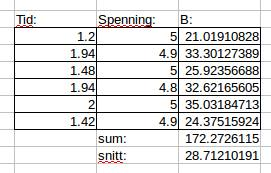
\includegraphics[scale=1]{gjennomforing/oppgave5.jpg}
\end{figure}
		
\end{document}